% 由目录数据排版部分标题页、章节、插图与部分结语。
\newcommand{\PendingBookPart}{}
\newcommand{\BookPart}[2]{\gdef\PendingBookPart{\BookPartPage{#1}{#2}}}
\newcommand{\BookPartPage}[2]{%
  \clearpage
  \refstepcounter{part}
  \addcontentsline{toc}{part}{#1：#2}
  \thispagestyle{empty}
  \begin{tikzpicture}[remember picture,overlay]
    \clip (current page.south west) rectangle (current page.north east);
    \IfFileExists{assets/part-art/part-\arabic{part}.png}{%
      \node[inner sep=0pt] at (current page.center)
        {\includegraphics[width=\paperwidth]{assets/part-art/part-\arabic{part}.png}};
    }{%
      \fill[Paper] (current page.south west) rectangle (current page.north east);
    }
    \node[anchor=north west,inner sep=0pt,
      font=\sffamily\fontsize{13}{18}\selectfont,text=Accent]
      at ([xshift=26mm,yshift=-35mm]current page.north west) {#1};
    \def\PartPageDisplayTitle{#2}
    \ifnum\value{part}=4
      \def\PartPageDisplayTitle{分布式购买系统的\\整体设计与工程架构}
    \fi
    \node[anchor=north west,inner sep=0pt,align=left,text width=158mm,
      font=\sffamily\bfseries\fontsize{30}{42}\selectfont,text=Ink]
      at ([xshift=26mm,yshift=-51mm]current page.north west) {\PartPageDisplayTitle};
    \draw[Accent,line width=1pt]
      ([xshift=26mm,yshift=-81mm]current page.north west)--++(21mm,0);
    \ifnum\value{part}=1
      \node[anchor=south,inner xsep=3mm,inner ysep=2mm,fill=Paper,fill opacity=.84,
        text opacity=1,text=Ink,font=\sffamily\fontsize{8}{11}\selectfont,
        align=center]
        at ([yshift=9mm]current page.south)
        {取意于霍贝玛《米德尔哈尼斯的林荫道》};
    \fi
    \ifnum\value{part}=2
      \node[anchor=south,inner xsep=3mm,inner ysep=2mm,fill=Paper,fill opacity=.84,
        text opacity=1,text=Ink,font=\sffamily\fontsize{8}{11}\selectfont,
        align=center]
        at ([yshift=9mm]current page.south)
        {取意于透纳《奇切斯特运河》};
    \fi
    \ifnum\value{part}=3
      \node[anchor=south,inner xsep=3mm,inner ysep=2mm,fill=Paper,fill opacity=.84,
        text opacity=1,text=Ink,font=\sffamily\fontsize{8}{11}\selectfont,
        align=center]
        at ([yshift=9mm]current page.south)
        {取意于莫奈《白杨树》};
    \fi
    \ifnum\value{part}=4
      \node[anchor=south,inner xsep=3mm,inner ysep=2mm,fill=Paper,fill opacity=.84,
        text opacity=1,text=Ink,font=\sffamily\fontsize{8}{11}\selectfont,
        align=center]
        at ([yshift=9mm]current page.south)
        {取意于卡纳莱托《从弗兰吉尼宫到圣马尔库奥拉广场的大运河》};
    \fi
  \end{tikzpicture}
  \null\clearpage
}
\newcommand{\BookChapter}[3]{%
  \ifnum#1>\LastReadyChapter\relax
  \else
    \PendingBookPart
    \gdef\PendingBookPart{}
    \setcounter{chapter}{\numexpr#1-1\relax}
    \ifnum#1=7\relax
      % 从第二部分起，为行内代码设置小幅词界。
      \renewcommand{\code}[1]{\allowbreak{\ttfamily\def\_{\textunderscore\allowbreak}##1}}
      \xeCJKsetup{CJKecglue={\hskip .22em plus .1em minus .08em}}
    \fi
    \chapter{#2}\label{chapter:#1}
    \def\CurrentChapterId{#1}
    \setcounter{section}{0}
    \ChapterArt{#1}
    \InputIfFileExists{chapters/#1-intro.tex}{}{}
    #3
    \ifnum#1=6\relax
      \clearpage
\chapter*{第一部分结语}
\addcontentsline{toc}{chapter}{第一部分结语}
\label{part:01-closing}

\begin{center}
  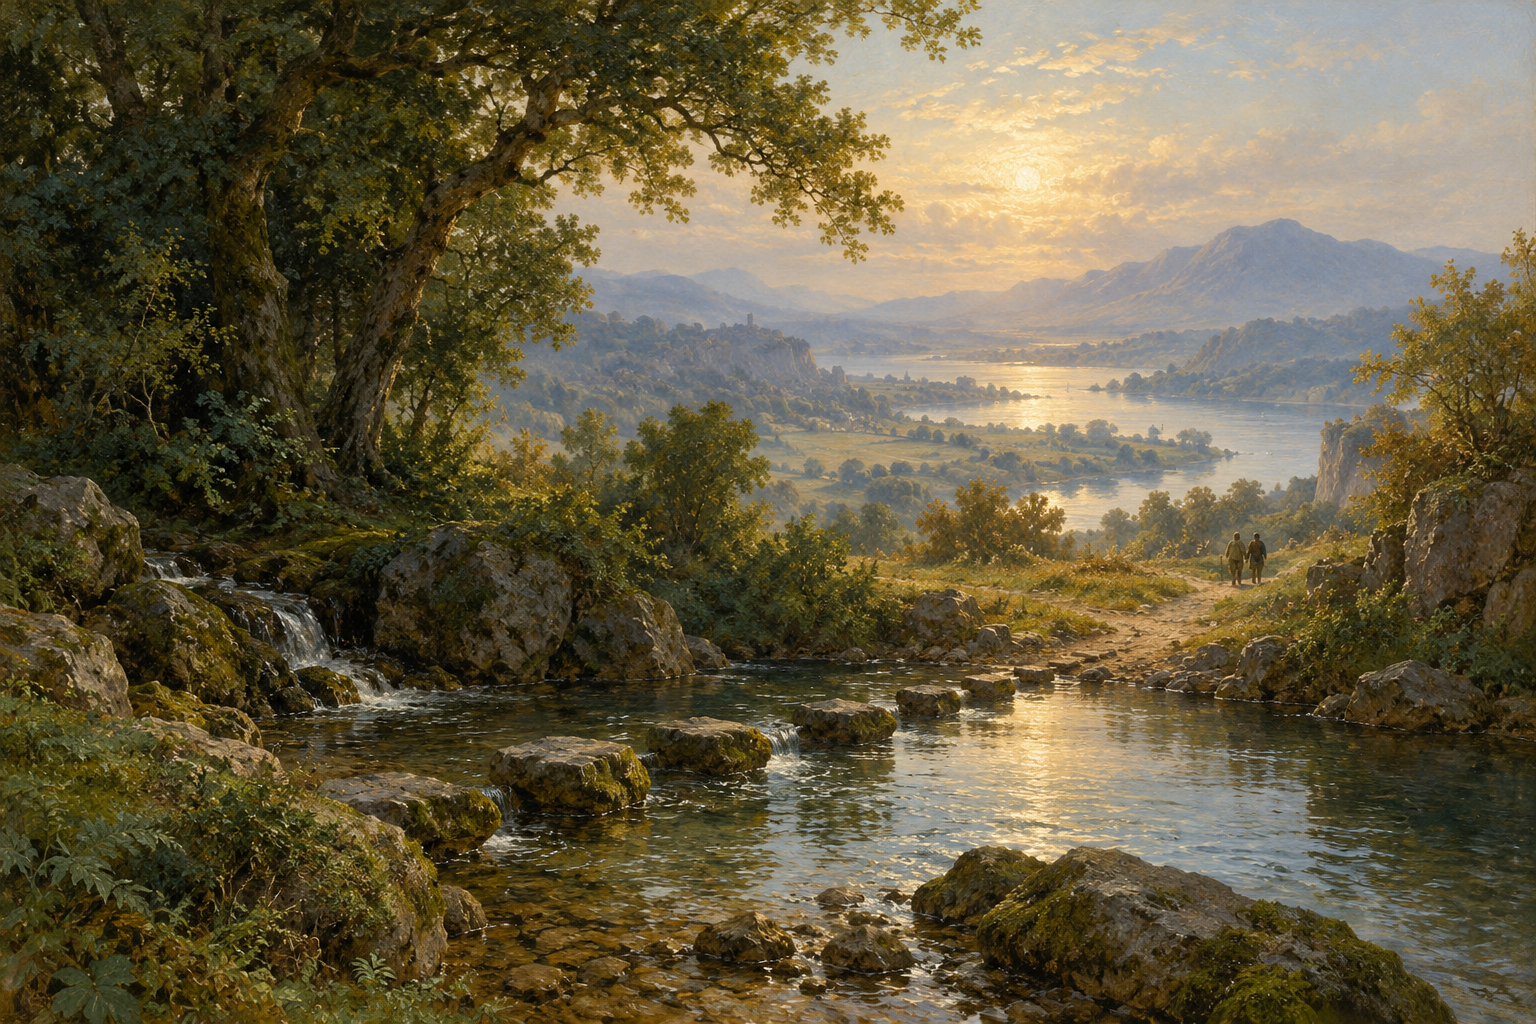
\includegraphics[width=\linewidth,height=.43\textheight,keepaspectratio]{assets/part-art/part-1-closing.png}
  \par\vspace{4pt}
  {\scriptsize\color{Muted}取意于透纳《渡溪》\par}
  \BookEpigraph{part1}
\end{center}

Alice 第一次购买时，账户从 10000 分减到 7000 分，订单和流水也已经保存。她等不到响应，再试一次，账户就变成了 4000 分。沿着这条历史，我们逐步修改了购买服务：先给购买保留身份，再让并发请求争取同一受理位置，最后把原结果与扣款一起保存。客户端依然可能超时，服务也依然可能退出；恢复程序现在有了可以查找和核对的记录。

这套处理从一次确认开始。客户端在发送以前保存完整身份、账户、动作、会话与已确认输入。同一次购买的后续尝试继续引用这条记录，再买一份则另建身份。这个区分关系到用户究竟授权了几次购买。服务收到的身份与输入，承载着调用方已经做出的区分；只有它们正确地对应到确认动作，服务端的受理规则才能对应到实际业务。

身份进入数据库以后，还要取得一项确定的关系：同一完整身份至多对应一条已提交购买。唯一约束检查这项关系，插入结果决定哪个事务继续处理。另一个请求遇到竞争，沿等待、回滚或读取原结果的路径继续。账户的条件更新负责检查余额并扣除金额，订单与流水保存这次成交的归属，完成记录则保存终态和原返回内容。它们各自承担的条件在共同提交处汇合，构成一份完整购买。

原结果保存了这份购买发生时的事实。P1 扣款以后是 7000 分，后来 P2 又把账户减到 4000 分，恢复 P1 仍会读回当次的 7000 分。账户查询负责报告当前余额，订单查询负责报告履约进度。把这些观察分开，调用方才能同时理解先前发生了什么，以及系统现在处于什么状态。结果中的编号、金额与终态也必须和实际订单、流水一致，稳定保存与真实关联共同支撑恢复。

提交和获知结果之间，仍可能相隔很久。一次请求在提交前退出，数据库撤销其内部修改，后来尝试可以重新取得身份；提交已经完成，恢复就沿原身份读取终态。提交确认尚未查明时，恢复者再次经过同一项身份检查，让数据库中的事务结局决定后续分支。客户端保留待确认状态，直到取得原结果或进入明确的核查流程。这段等待期间，已经成立的业务事实继续存在于数据库中。

第一部分的论证依赖明确的范围：购买与本地扣款由同一数据库事务完成，所有相关写入经过规定的仲裁，已确认提交在所讨论的故障后继续保留；恢复使用原身份、原输入和可解释的结果版本，记录在承诺的期限内保持可读。第六章把资金动作限定为购买扣款，因此余额只会保持或下降，余额不足的判断也能在这个模型中安排到终态提交处。加入充值以后，需要重新核对拒绝判断与提交之间的并发关系。操作集合改变，原先依赖的条件也随之改变。

期限同样属于设计的一部分。第一部分在会话有效、记录保留的范围内恢复；期限结束后，第三章的关闭与在途保护边界继续约束清理。持续重试还需要实际机会：数据库恢复可用，旧事务终结，恢复者得到运行，至少一次完整结果能够到达并保存。一次操作已经提交，与客户端最终知道它已经提交，是两个分别需要条件支持的目标。

我们用三种方法检查这些关系。逐步论证说明允许的迁移怎样保持不变量；有界模型展开有限范围内的交错，并让错误方案产生可复核的反例；实际中断实验检查选定位置的进程退出与数据库恢复。它们让设计中的假设、实现中的步骤和观察到的事实能够相互核对。新的故障类型或写入路径进入系统以后，也可以沿这些关系追查：哪一条不变量受影响，哪项前提已经改变，恢复者还能读到什么证据。

接下来，购买服务会把扣款交给另一个系统。对方可以独立完成扣款，本地数据库也有自己的提交结局。第一部分已经连在一起的身份、业务效果与完成记录，将分布在两个提交边界内。我们要继续处理同一个问题：响应丢失以后，恢复者依据哪些持久事实，决定等待、查询或继续执行。

    \fi
    \ifnum#1=10\relax
      \clearpage
\chapter*{第二部分结语}
\addcontentsline{toc}{chapter}{第二部分结语}
\label{part:02-closing}

\begin{center}
  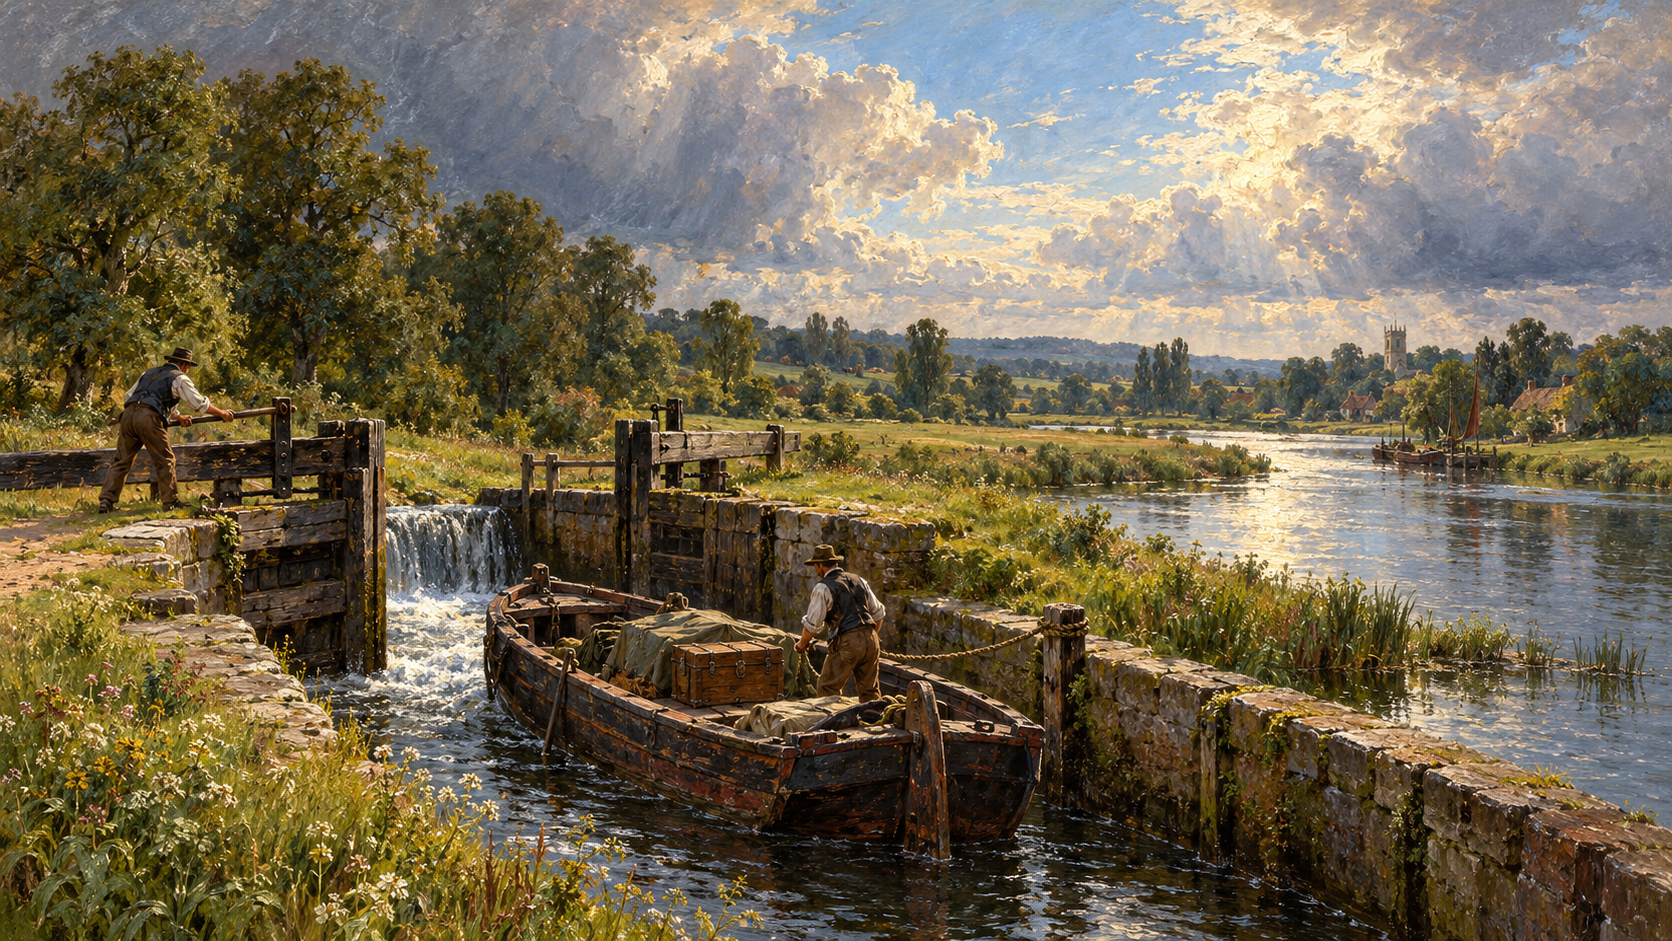
\includegraphics[width=\linewidth,height=.43\textheight,keepaspectratio]{assets/part-art/part-2-closing.png}
  \par\vspace{4pt}
  {\scriptsize\color{Muted}取意于康斯太勃尔《水闸》\par}
  \BookEpigraph{part2}
\end{center}

Alice 的购买已经跨过几次进程退出。平台扣去 3000 分，购买服务一度还在等待付款；后来订单与通知一起保存，消息也可能发过两次。同一 EV1 先后到达履约处理器三次，后两次都找到原来的 F1。把这段历史按系统分开看，每个系统都保存着自己已经确认的事实，恢复程序沿这些事实接续下一段工作。

第一处变化发生在 A。购买服务先保存 P1、C1 与固定平台身份，后来工作者才能用原输入继续付款。E 已在平台提交、R 尚未在购买库完成时，本地等待准确表达了证据尚缺的阶段。查询、回调与对账逐步补足这份证据，R 再把原结果和唯一订单共同保存。超时留下的两个分支由原身份关联，服务可以继续查询和恢复，而无须从超时本身猜出平台是否已经扣款。

T1 把持续运行的责任留在了数据库。进程失联以后，扫描器根据状态与到期条件重新发现它；新的领取取得新的代次，调度入口据此拒绝旧工作者的回写。与此同时，一份可信的旧平台响应依然可能说明 X1 已经存在。授权谁安排下一轮工作，与确认付款发生了什么，分别在自己的入口核验。到了独立资源，接收者还要把代次检查、水位推进和实际修改共同仲裁，才能拒绝迟到旧写。同代次不同业务进度的顺序，则由另外保存的业务版本解释。

通知把相似的问题带到新的边界。R 可以原子保存付款结论与 EV1，代理稍后独立受理消息。发布确认丢失以后，PA2 可能把同一 EV1 再送一次，因此消费者继续携带原事件身份。Q 用 I 恢复一次接收，用 B 约束初次履约，把真实 F 与本地结果、回报责任一起提交。另一份合法购买取得另一 O，两个不同事件也可能报告同一个 O；两层身份让这两种情况得到各自正确的处理。

\clearpage
\CTenFigure{part02-responsibility}{上游先保存待办与下游身份，后续接收者提交自己的效果及继续依据}{fig:part02-responsibility}

这些步骤共有一项构造方法。先找到当前系统能够原子保存的那组事实，把下一段工作的原输入、稳定身份和待办放进这次提交。接收者取得工作以后，在自己能控制效果的位置仲裁重复、核对输入并保存结果。发送者缺少确认时，从原记录继续；收到足够证据时，结束本段待办。每次转交都留下可查的位置，进程和连接的寿命便可以短于整项业务的寿命。

这条方法也限定了能够作出的承诺。外部平台缺少固定身份保护时，本地唯一行数无法限制平台扣款数。代理确认以后若允许无证据删除消息，消费者可能失去继续输入。仓储请求已经发出却无法查明结果时，持久核查保住原映射和处置责任，发货结局则等待相应证据。安全保证逐段依赖具体仲裁，最终完成逐段依赖记录可读、实际调度、网络机会与有依据的处置。

本地回滚的作用域始终清楚。R 回滚撤销购买库内尚未提交的订单、结果和事件，平台 E 继续保留已完成的收款。Q 回滚撤销履约库内的候选，代理中的副本继续按自己的规则存放。后来需要退款、补发或更正时，它们各自取得业务授权、身份和恢复路径。已经确认的付款与履约成为这些后续动作的依据。

到这里，每一段恢复都用到了已提交记录的延续性：P/C 的固定映射、任务代次、资源高水位、EV 的原快照，以及 I/B/F 的绑定。这个条件在前面采用的故障模型中成立，接下来的系统变化会直接检验它。若新主库缺少先前确认的购买，旧请求会再次找到空位置；若去重结果已经回收，迟到副本可能失去拒绝依据；若备份把任务代次恢复到昨天，旧消息和新领取又会共享过去用过的数字。

第三部分从这些具体历史继续：复制怎样保住已承诺的事实，记录在什么条件下才可遗忘，以及恢复旧历史以后，服务要取得哪些外部证据才能重新开放入口。一次购买的身份继续沿用，变化的是恢复者还能依赖哪些保存下来的历史。

    \fi
    \ifnum#1=15\relax
      \clearpage
\chapter*{第三部分结语}
\addcontentsline{toc}{chapter}{第三部分结语}
\label{part:03-closing}

\begin{center}
  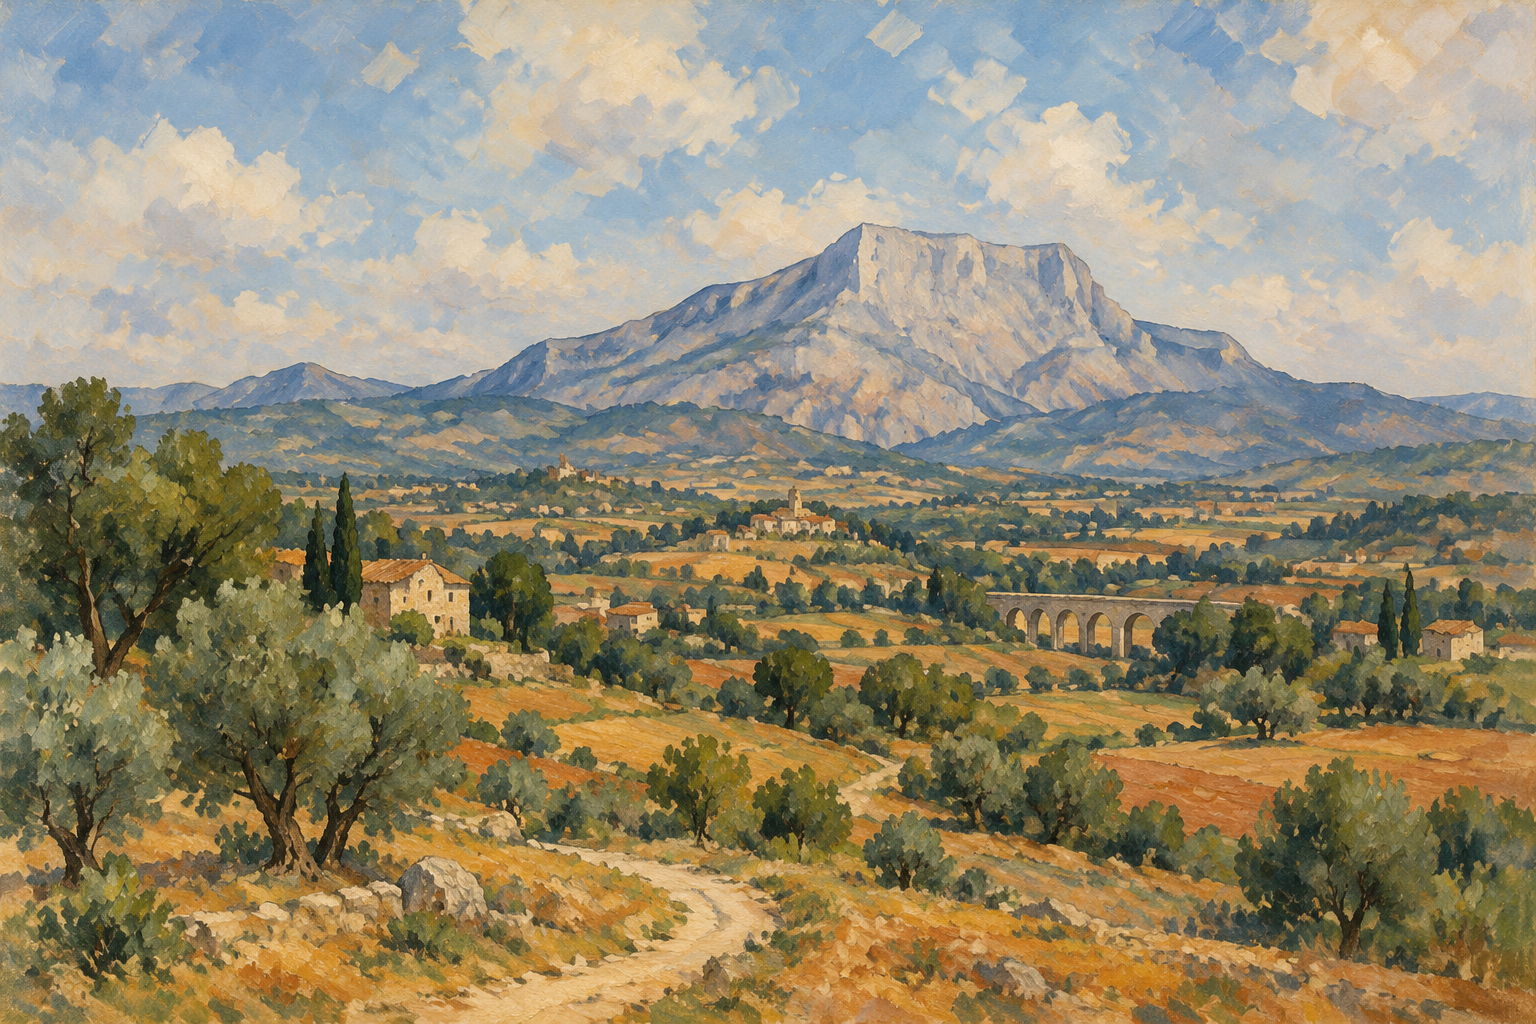
\includegraphics[width=\linewidth,height=.43\textheight,keepaspectratio]{assets/part-art/part-3-closing.png}
  \par\vspace{4pt}
  {\scriptsize\color{Muted}取意于塞尚《圣维克多山》\par}
  \BookEpigraph{part3}
\end{center}

Alice 的原购买曾经只在一台服务的事务中出现。到了这一部分，它已经随日志传到接班副本，进入快照，也可能在购买库的旧备份中消失。平台上的 X1 与履约库里的 F501 继续存在，恢复者要把它们接回原来的 P1/C1/O1。业务的过去分布在不同保存位置，每一个位置都有自己的提交与恢复边界。

复制首先延续已经确认的决定。状态机按提交顺序应用命令，把身份绑定、原输入、结果、会话资格和应用边界一起保存。另一副本接班以后，重复命令即使位于新的日志位置，也会找到原 $S$。快照压缩了日志表示，原购买及其拒绝重复的依据继续属于恢复后的状态。

记录回收改变了保存这些区别的方式。E1 关闭以后，旧购买提交入口结束准入，原来的逐项结果可以按规则缩减，关闭决定和从未重用的登记进度继续保存。已经接受的 C1/T1 则沿原关联完成核查。平台逐键窗口、旧在途请求与可取得的终结证据共同决定发送何时结束，固定的本地截止把客户端能够重新提交的范围写清楚。

状态表达也能改变需要传播的历史。标签按并集合并，重复到达后集合保持；带来源标记的删除把已经观察到的新增与并发新增区分开来。资金增量、退款额度和首次发货依赖另外的业务条件。把同一笔 1000 退款传播两次，与接受两项各 1000 的退款，在原 RF 上有不同含义。已经形成的事实可以继续合并，首次责任由身份、授权与共同仲裁决定。

\CFifteenFigure{ch15-22-part3-history}{保存决定、关闭旧准入和恢复原关系共同延续已经承担的业务责任}{fig:part03-history}

主动回退购买库时，独立 J 保存的原关系提供了另一条恢复路径。恢复者先从 $S$ 取得原 P1/C1/T1，再用原范围和 \code{pay-C1} 核对 X1，并以 $R_J$ 中的原编号、结果和 EV1 物化本地记录。已有行的完整内容参与核对，冲突使本批写入与物化边界一起回滚。目录把恢复资格与新意图准入连接起来，入口依据已经完整恢复的范围开放。

退款把这条保存链延伸到新责任。RF1 的平台结果未知时，原金额继续占用 X1 的退款额度；成功证据到达后，占用转为已退，足够最终拒绝则释放额度。旧备份删除本地投影以后，J 中的绑定与预占依然能够重建。净资金、原购买成功和当前退款进度各自有确定的数据来源，查询把这些事实组合到同一项业务上。

这些机制进入完整系统以后，会同时争用目录、数据库、任务队列和外部平台。架构设计要先给出它们共同构成的系统：谁拥有每类事实，哪些调用跨过事务域，流量如何到达权威位置，恢复者怎样发现并接续已经接受的责任。在这个整体中，再决定每个组件的数据、接口、容量与故障处理。第四部分由此转向完整系统架构，让购买、付款、退款和履约的保证在同一部署中各有承担位置。
\FloatBarrier

    \fi
    \ifnum#1=21\relax
      \clearpage
\chapter*{第四部分结语}
\addcontentsline{toc}{chapter}{第四部分结语}
\label{part:04-closing}

\begin{center}
  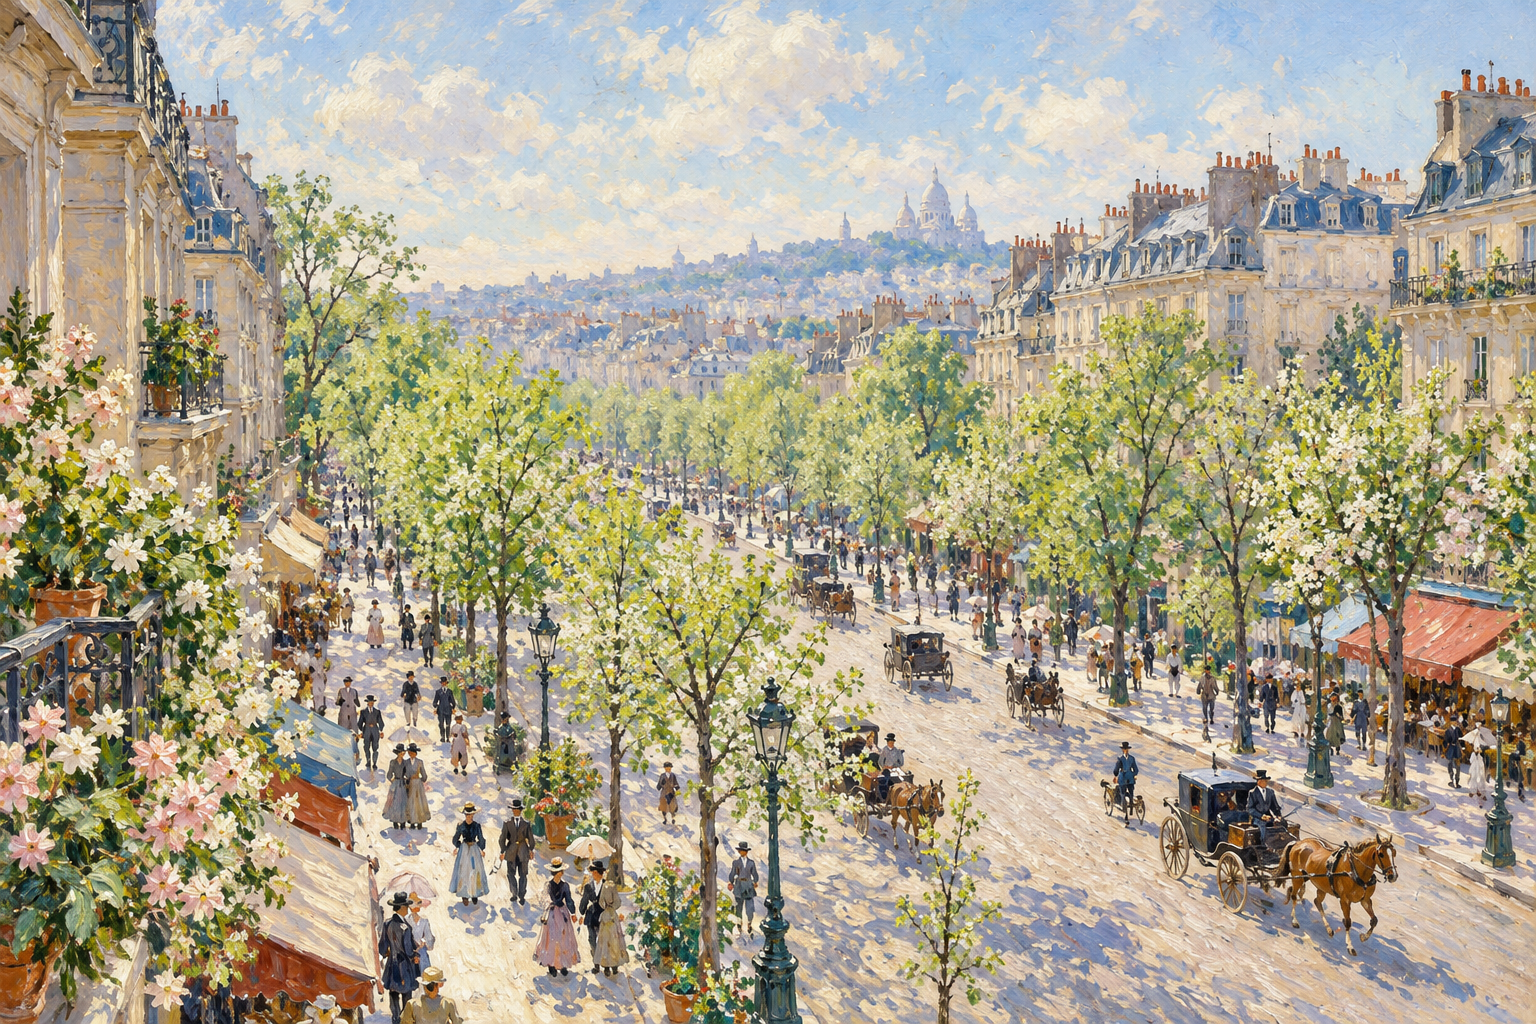
\includegraphics[width=\linewidth,height=.35\textheight,keepaspectratio]{assets/part-art/part-4-closing.png}
  \par\vspace{4pt}
  {\scriptsize\color{Muted}取意于卡米耶·毕沙罗《蒙马特大道，春天的早晨》\par}
  \BookEpigraph{part4}
\end{center}

第四部分把购买服务展开为一套共同运行的系统。入口根据目录找到购买权威，库存组保存资源预留，支付平台掌管实际收款，消息域传递事件，消费事务库保存履约与发运意图。每个组件有自己的接口、保存状态和故障处理，原购买的关联把这些位置接到同一条业务链上。沿链查看一次处理，可以找到当前决定由谁作出、结果保存在哪里、接下来的工作由谁承担。

购买权威保存完整身份到实际 P/C/T 的绑定，以及随后形成的原结果、订单与 EV。分区复制状态机按提交顺序共同修改这些关系，也可以选择由分布式 SQL 的事务与约束承担相应修改。复制保存确认过的决定，快照包含会话、结果、编号进度和未决责任。读取原结果时，服务沿原绑定返回当次事实，当前履约与退款查询则继续读取各自的新进度。

控制面保存逻辑分区当前的位置和执行资格。目录更新以后，入口缓存逐步刷新，实际接收写入的组核验归属与代次。协调服务的版本、会话和通知帮助应用接续配置，业务资源再在实际修改处检查资格。查询缓存则从权威事实形成可重建观察，过期、淘汰和节点切换以后，按保存的来源与版本重建所需状态。

外部付款从受理时保存的 C/T 继续。工作者根据领取代次安排发送、查询与回填，发送使用已保存的平台、商户范围、环境、动作和 \code{pay-C}。X1 已经完成而本地尚未取得确定证据时，付款保持未知。查询、可信回调和对账逐步核对原收款，权威随后固定结果、订单与事件。平台只提供时点查询，或原键保护期和在途请求尚有歧义时，原 C 留在持续核查路径，调度依据已保存状态安排后续查询。

联合库存预留在各库存组之间组织共同决定。参与者保存准备占用，协调者持久保存 commit 或 abort，恢复者把原决定送到各组。参考流程等待全部必需参与者完成以后，才开启原 C/T 的付款资格。库存占用、协调者决定和付款资格都进入各自的复制状态，接班者据此继续传播决定或推进付款。

付款形成的原 EV 可以经过重复发布和重投。RabbitMQ 的路由、队列与确认，Kafka 的分区日志、事务与消费位置，分别规定消息域内部的处理。消费者在本地事务中保存 I/B/F、结果和 dispatch 意图。消息保留期有限时，持久消费交接回执把 F 的接受事实送回购买权威，更新履约进度并结束原事件的补发责任，实际发运则沿原 dispatch 继续查询外部平台，把确定结果接回相应的履约记录。

退款在这条链上建立新的 RF，关联原 C 与 X1。收款 3000 分，成功退款 1000 分，另有 1500 分未知，后续最多再占用 500 分。调度转入人工核查以后，未知的 1500 分继续保留占额，取得确定证据后再转换或释放。财务、客服与用户查询由此可以同时解释原购买成功、当前净资金与退款进度。

存储与计算组件也参与这些保存和接续。块与对象保存图像、日志和文件，发布协议确定哪个版本或文件集合已经生效。批处理以固定输入组织重执行，用提交结果确定有效输出；任务、Actor 与函数运行时则按各自规则调度和恢复执行。持久工作流保存步骤位置，付款步骤从原平台关联继续。推测执行、共识优化和地域读协议调整具体等待，部署为相应日志、检查点、资格和证据安排保存与恢复资源。

完整分区迁移把这些业务关系交给新的承载组。参考首版先闭合 prepared 库存与未完成协调者事务，再冻结图像并切换目录，已受理的外部责任随原关联交接。旧备份恢复则先找回旧身份的绑定和较新的外部证据，或者持久关闭歧义范围，再开放相应入口。缓存重建、快照下载、日志接续和任务扫描分别占用网络、磁盘与执行能力，恢复放量沿这些依赖分批推进。

容量设计最后把整套架构连到实际运行。平台恢复使 T 下降，同时可能产生更多 EV 与消费积压。调度按整条链的净排空能力安排新流，为原结果查询、确定证据回填、事务决定恢复和事件交接保留预算。观测从原身份找到各段责任，再显示积压年龄、最近证据和下一步动作，值守者便能据此限制新增负担、调整恢复份额或发起核查。
\FloatBarrier

    \fi
  \fi
}
\newcommand{\BookSection}[1]{%
  \section{#1}\label{section:\CurrentChapterId-\arabic{section}}
  \edef\SectionSource{chapters/\CurrentChapterId-\arabic{section}.tex}
  \InputIfFileExists{\SectionSource}{}{%
    \PackageError{book}{Missing section source: \SectionSource}{Create the real section text before switching to body mode.}}
}

\newcommand{\ChapterArt}[1]{%
  \IfFileExists{assets/chapter-art/chapter-#1.png}{%
    \begin{center}
      \includegraphics[width=\linewidth,height=.43\textheight,keepaspectratio]{assets/chapter-art/chapter-#1.png}
      \par\vspace{4pt}
      {\scriptsize\color{Muted}\ChapterArtCredit{#1}\par}
      \BookEpigraph{#1}
    \end{center}
    \vspace{2mm}
  }{\PackageError{book}{Missing chapter art for #1}{Generate and review chapter opening art before publication.}}
}
\newcommand{\ChapterArtCredit}[1]{%
  \ifnum#1=1
    取意于伦勃朗《布商同业公会的理事》
  \fi
  \ifnum#1=2
    \strut
  \fi
  \ifnum#1=3
    \strut
  \fi
  \ifnum#1=4
    \strut
  \fi
  \ifnum#1=5
    \strut
  \fi
  \ifnum#1=6
    \strut
  \fi
  \ifnum#1=7
    取意于维米尔《写信的女子与女佣》
  \fi
  \ifnum#1=8
    取意于伦勃朗《夜巡》
  \fi
  \ifnum#1=9
    取意于维米尔《情书》
  \fi
  \ifnum#1=10
    取意于伦勃朗《布商公会理事》
  \fi
  \ifnum#1=11
    取意于拉斐尔《雅典学院》
  \fi
  \ifnum#1=12
    取意于维米尔《天文学家》
  \fi
  \ifnum#1=13
    取意于保罗·克利《城堡与太阳》
  \fi
  \ifnum#1=14
    取意于透纳《被拖去解体的战舰特米雷尔号》
  \fi
  \ifnum#1=15
    取意于维米尔《持天平的女人》
  \fi
  \ifnum#1=16
    取意于彼得·勃鲁盖尔《巴别塔》
  \fi
  \ifnum#1=17
    取意于葛饰北斋《神奈川冲浪里》
  \fi
  \ifnum#1=18
    取意于萨尔瓦多·达利《记忆的永恒》
  \fi
  \ifnum#1=19
    取意于保罗·塞尚《圣维克多山》
  \fi
  \ifnum#1=20
    取意于克劳德·莫奈《圣拉扎尔火车站》
  \fi
  \ifnum#1=21
    取意于保罗·西涅克《红色浮标》
  \fi
}
